The full Promela model, with the LTL properties for the CWP, is in a public Github repository \cite{repo}. The \emph{README.md} file in the repository summarizes its content and how to reproduce the proof certificate for the model. The actual model is divided into three files: the CWP object state, the CWP LTL properties, and the BPMN workflow model. A script, \emph{short-verify.sh}, combines the three files to create the final Promela model and then runs SPIN on all twenty properties.

\begin{figure}
  \begin{center}
    \begin{tabular}{c}
      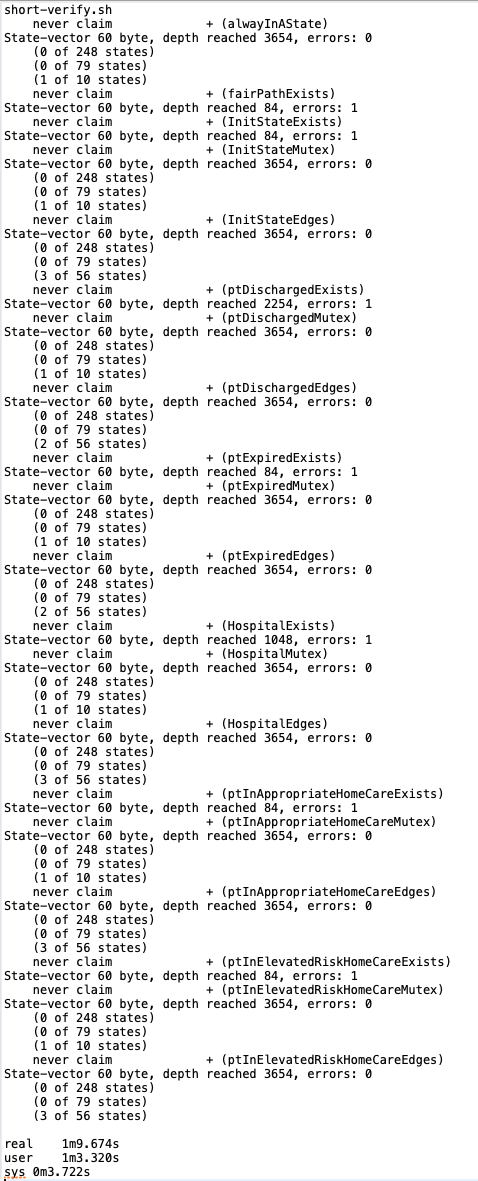
\includegraphics[scale=0.5]{proof.png}
    \end{tabular}
  \end{center}
\caption{The verification results from the SPIN model checker.}
\label{fig:proof}
\end{figure}

Verification takes around three to four minutes on an Intel Core i7 laptop with 16 Gb of RAM. It is not taxing the system in any way. The output from the script is shown in \figref{fig:proof}. The output names the property being verified (e.g., the \emph{never claim}). Following the named property, there is a  summary of the verification effort and what was proved. The critical value being the reported errors.

All the existential properties (i.e., the properties ending with \emph{Exists}) should result in an error. The error is the existential witness. All the other properties should pass with no errors. The output of the script includes not just the error report but the coverage summary of the processes and properties. The first two entries pertain to the clinician and patient-caregiver processes. There should never be uncovered states in these processes. Uncovered states means that there are unreachable behaviors in the model---not good. The third entry is the property being verified. It is not unusual to have uncovered states here when there is no reported error since the error behavior is not found in the model---good.